\section{moeo\-Entropy\-Metric$<$ EOT $>$ Class Template Reference}
\label{classmoeoEntropyMetric}\index{moeoEntropyMetric@{moeoEntropyMetric}}
The entropy gives an idea of the diversity of a Pareto set relatively to another Pareto set.  


{\tt \#include $<$moeo\-Entropy\-Metric.h$>$}

Inheritance diagram for moeo\-Entropy\-Metric$<$ EOT $>$::\begin{figure}[H]
\begin{center}
\leavevmode
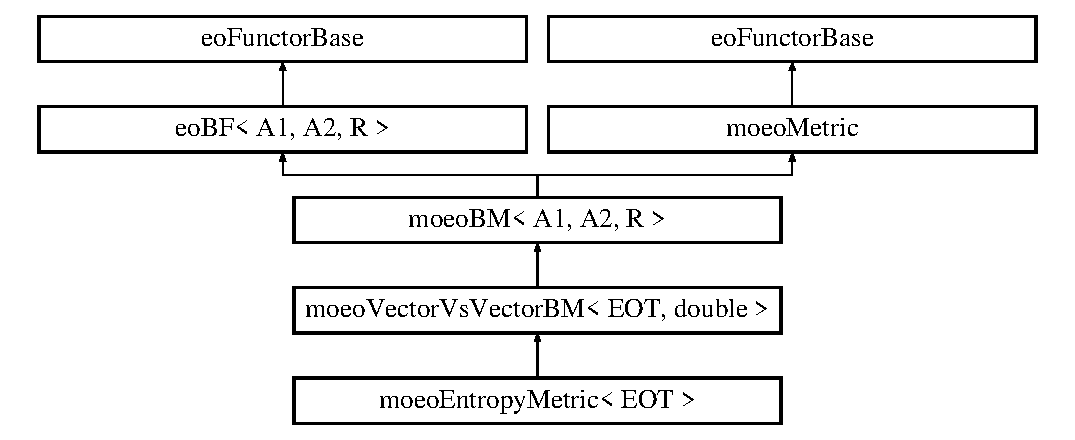
\includegraphics[height=5cm]{classmoeoEntropyMetric}
\end{center}
\end{figure}
\subsection*{Public Types}
\begin{CompactItemize}
\item 
typedef EOT::Fitness {\bf EOFitness}\label{classmoeoEntropyMetric_306b72d2236de1ecbae986c65490a8fe}

\begin{CompactList}\small\item\em The fitness type of a solution. \item\end{CompactList}\end{CompactItemize}
\subsection*{Public Member Functions}
\begin{CompactItemize}
\item 
double {\bf operator()} (const std::vector$<$ {\bf EOFitness} $>$ \&\_\-set1, const std::vector$<$ {\bf EOFitness} $>$ \&\_\-set2)
\begin{CompactList}\small\item\em Returns the entropy of the Pareto set '\_\-set1' relatively to the Pareto set '\_\-set2'. \item\end{CompactList}\end{CompactItemize}
\subsection*{Private Member Functions}
\begin{CompactItemize}
\item 
void {\bf remove\-Dominated} (std::vector$<$ {\bf EOFitness} $>$ \&\_\-f)\label{classmoeoEntropyMetric_3252e7534b1ceb1317936c5d2b3abcbe}

\item 
void {\bf prenormalize} (const std::vector$<$ {\bf EOFitness} $>$ \&\_\-f)\label{classmoeoEntropyMetric_c9f0c65b4de69accbfb42486f6445cb0}

\item 
void {\bf normalize} (std::vector$<$ {\bf EOFitness} $>$ \&\_\-f)\label{classmoeoEntropyMetric_bc32468b148a0da4eb21a9fc14dfafae}

\item 
void {\bf compute\-Union} (const std::vector$<$ {\bf EOFitness} $>$ \&\_\-f1, const std::vector$<$ {\bf EOFitness} $>$ \&\_\-f2, std::vector$<$ {\bf EOFitness} $>$ \&\_\-f)\label{classmoeoEntropyMetric_2de60a0e6be362f074b50e6b455152ab}

\item 
unsigned {\bf how\-Many\-In\-Niche\-Of} (const std::vector$<$ {\bf EOFitness} $>$ \&\_\-f, const {\bf EOFitness} \&\_\-s, unsigned \_\-size)\label{classmoeoEntropyMetric_a9369be315e139ebdf19fac09ad0563f}

\item 
double {\bf euclidian\-Distance} (const {\bf EOFitness} \&\_\-set1, const {\bf EOFitness} \&\_\-to, unsigned \_\-deg=2)\label{classmoeoEntropyMetric_34f825ce7c53132f7218483130da8652}

\end{CompactItemize}
\subsection*{Private Attributes}
\begin{CompactItemize}
\item 
std::vector$<$ double $>$ {\bf vect\_\-min\_\-val}\label{classmoeoEntropyMetric_d4046a304badfe78aa35b2d57938ffe9}

\item 
std::vector$<$ double $>$ {\bf vect\_\-max\_\-val}\label{classmoeoEntropyMetric_af0ae9645bdbb993de4bc990a0a08883}

\end{CompactItemize}


\subsection{Detailed Description}
\subsubsection*{template$<$class EOT$>$ class moeo\-Entropy\-Metric$<$ EOT $>$}

The entropy gives an idea of the diversity of a Pareto set relatively to another Pareto set. 

(Basseur, Seynhaeve, Talbi: 'Design of Multi-objective Evolutionary Algorithms: Application to the Flow-shop Scheduling Problem', in Proc. of the 2002 Congress on Evolutionary Computation, IEEE Press, pp. 1155-1156) 



Definition at line 23 of file moeo\-Entropy\-Metric.h.

\subsection{Member Function Documentation}
\index{moeoEntropyMetric@{moeo\-Entropy\-Metric}!operator()@{operator()}}
\index{operator()@{operator()}!moeoEntropyMetric@{moeo\-Entropy\-Metric}}
\subsubsection{\setlength{\rightskip}{0pt plus 5cm}template$<$class EOT$>$ double {\bf moeo\-Entropy\-Metric}$<$ EOT $>$::operator() (const std::vector$<$ {\bf EOFitness} $>$ \& {\em \_\-set1}, const std::vector$<$ {\bf EOFitness} $>$ \& {\em \_\-set2})\hspace{0.3cm}{\tt  [inline]}}\label{classmoeoEntropyMetric_58136405dfed951efa340ddf541c29fd}


Returns the entropy of the Pareto set '\_\-set1' relatively to the Pareto set '\_\-set2'. 

\begin{Desc}
\item[Parameters:]
\begin{description}
\item[{\em \_\-set1}]the first Pareto set \item[{\em \_\-set2}]the second Pareto set \end{description}
\end{Desc}


Definition at line 38 of file moeo\-Entropy\-Metric.h.

References moeo\-Entropy\-Metric$<$ EOT $>$::compute\-Union(), moeo\-Entropy\-Metric$<$ EOT $>$::how\-Many\-In\-Niche\-Of(), moeo\-Entropy\-Metric$<$ EOT $>$::normalize(), moeo\-Entropy\-Metric$<$ EOT $>$::prenormalize(), and moeo\-Entropy\-Metric$<$ EOT $>$::remove\-Dominated().

The documentation for this class was generated from the following file:\begin{CompactItemize}
\item 
moeo\-Entropy\-Metric.h\end{CompactItemize}
